\chapter{\textit{DYNAMIC TIME WARPING}} \label{cha:dtw}

O \textit{Dynamic Time Warping} (DTW) \cite{tavenard.blog.dtw} é um algoritmo amplamente utilizado para medir a similaridade entre duas sequências temporais que podem variar em velocidade, tempo ou comprimento. Sua principal aplicação está em áreas como reconhecimento de fala, análise de séries temporais, bioinformática e visão computacional. Neste trabalho, essa técnica é utilizada para comparação entre as curvas que representam as características faciais dos indivíduos, permitindo identificar as mesmas pessoas em diferentes momentos ou condições.

\section{Introdução}

Este algoritmo surgiu como uma solução para o problema de comparação entre sequências temporais que apresentam distorções no eixo do tempo. Diferente da distância Euclidiana, que compara ponto a ponto, o DTW permite alinhar dinamicamente duas sequências, encontrando o menor custo de distorção temporal necessário para que elas se assemelhem.

Considere duas sequências temporais:
\begin{equation}
    X = (x_1, x_2, \ldots, x_n) \quad \text{e} \quad Y = (y_1, y_2, \ldots, y_m),
\end{equation}
onde \(X\) e \(Y\) são as sequências a serem comparadas, com \(n\) e \(m\) sendo seus respectivos comprimentos.

O algoritmo de DTW constrói uma matriz de custo acumulado \(D\) de dimensão \(n \times m\), na qual cada elemento \(D(i, j)\) representa o custo mínimo acumulado para alinhar os primeiros \(i\) elementos de \(X\) com os primeiros \(j\) elementos de \(Y\).

O alinhamento entre os primeiros elementos das sequências ocorre diretamente na célula \(D(1,1)\), definida como:

\begin{equation}
    D(1,1) = d(x_1, y_1),
\end{equation}
onde \(d(x_1, y_1)\) é a distância entre os primeiros elementos de cada sequência, usualmente calculada por uma métrica como a distância Euclidiana.

Em seguida, são preenchidas a primeira linha e a primeira coluna da matriz. Nessas bordas, o caminho de alinhamento é único (ou apenas vertical ou apenas horizontal), o que resulta em uma soma cumulativa de distâncias. Assim, a inicialização segue as seguintes fórmulas:

\begin{align}
    D(i,1) &= d(x_i, y_1) + D(i-1,1), \quad \text{para } i = 2, \ldots, n, \\
    D(1,j) &= d(x_1, y_j) + D(1,j-1), \quad \text{para } j = 2, \ldots, m.
\end{align}

Essa etapa garante que todas as possíveis trajetórias de alinhamento que passam pelas extremidades da matriz possam ser consideradas no cálculo recursivo subsequente.

\subsubsection*{Preenchimento recursivo da matriz}

A partir de \(i = 2\) e \(j = 2\), a matriz é preenchida utilizando a fórmula recursiva do DTW:

\begin{equation}
    D(i, j) = d(x_i, y_j) + \min \begin{cases}
        D(i-1, j), \\
        D(i, j-1), \\
        D(i-1, j-1),
    \end{cases}
    \quad \text{para } i \geq 2 \text{ e } j \geq 2.
\end{equation}

Essa relação computa o custo acumulado de alinhar \(x_i\) com \(y_j\). O valor final \(D(n, m)\) representa o custo total do alinhamento ótimo entre as duas sequências temporais.


A \autoref{fig:dtw_intro} ilustra o conceito de alinhamento dinâmico, mostrando como o DTW pode distorcer o eixo do tempo para alinhar duas sequências temporais que, à primeira vista, parecem diferentes.

\begin{figure}[h!]
    \centering
    \caption{ALINHAMENTO DINÂMICO.}
    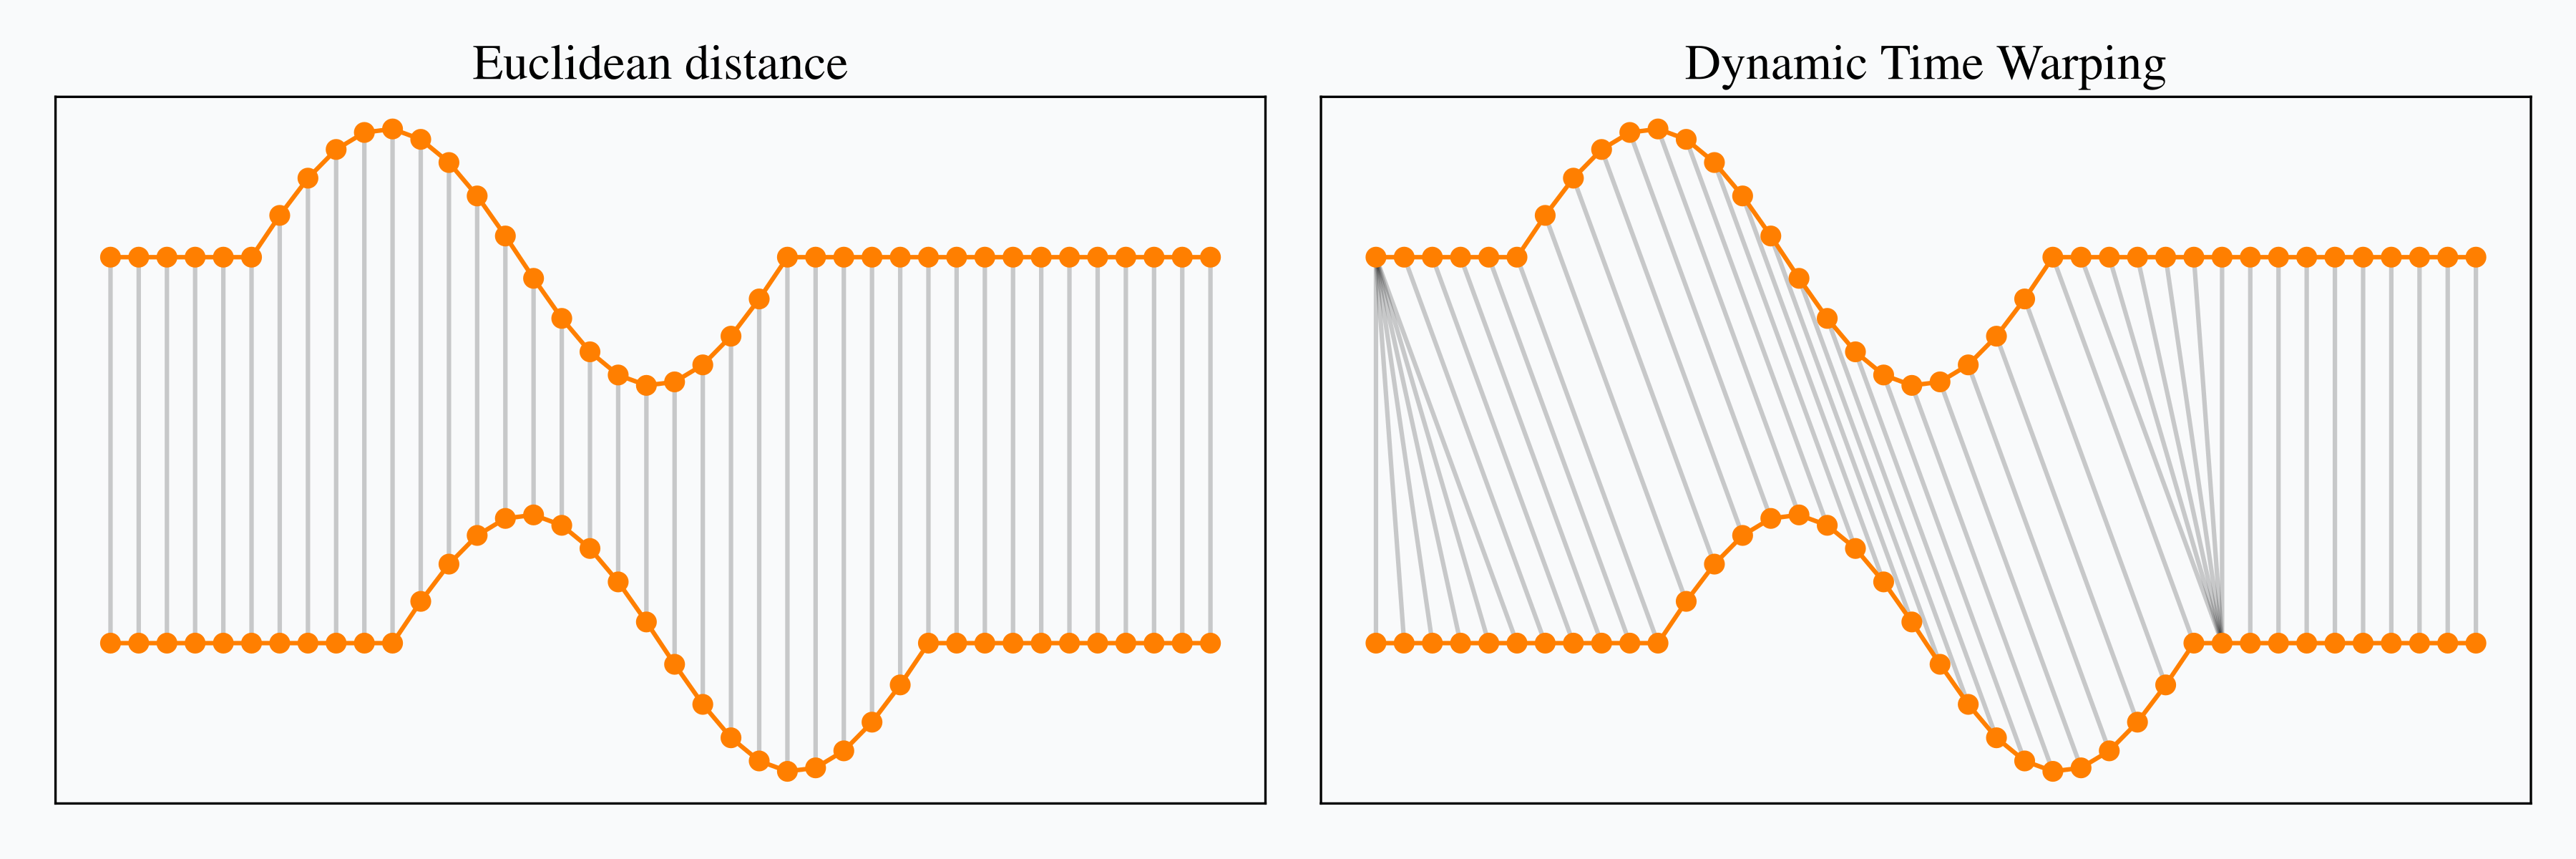
\includegraphics[width=0.8\textwidth]{fig/dtw_vs_euc.png}
    \legend{FONTE: \cite{tavenard.blog.dtw}}
    \label{fig:dtw_intro}
\end{figure}

\section{Vantagens e Desvantagens}

O método apresenta diversas vantagens em relação a outras métricas de distância, como a distância Euclidiana. Entre elas, destacam-se:
\begin{itemize}
    \item \textbf{Robustez a variações de tempo}: É capaz de lidar com sequências que apresentam variações na velocidade ou no comprimento, permitindo comparações mais precisas.
    \item \textbf{Alinhamento dinâmico}: Encontra o melhor alinhamento entre as sequências, minimizando o custo total de distorção temporal.
    \item \textbf{Versatilidade}: Funciona bem em sinais unidimensionais e multidimensionais, sendo aplicável em diversas áreas como reconhecimento de padrões e análise de séries temporais.
\end{itemize}

No entanto, o DTW também possui desvantagens:
\begin{itemize}
    \item \textbf{Complexidade computacional}: O algoritmo tem complexidade \(O(n \cdot m)\), o que pode ser um limitante para sequências muito longas.
    \item \textbf{Sensibilidade a ruídos}: Pode ser afetado por ruídos nas sequências, o que pode levar a alinhamentos incorretos.
\end{itemize}


\section{Justificativa para o seu uso}

Neste trabalho, o DTW foi utilizado por ser uma técnica adequada para comparar sequências que representam características espaciais extraídas de contornos faciais utilizando um algoritmo simples. As curvas resultantes dessas características podem variar em comprimento e forma devido a diferentes condições de iluminação, expressões faciais ou ângulos de captura. Esse método permite alinhar essas curvas de forma dinâmica, possibilitando uma comparação mais precisa entre elas.

Além disso, este trabalho baseia-se na abordagem proposta por \citet{DTW_LSTM}, que demonstraram a eficácia do uso do algoritmo DTW na comparação da variação das cores dos \textit{pixels} ao longo do vetor. Os autores obtiveram acurácias de 100\%, 94\% e 70\% em diferentes cenários experimentais, evidenciando a robustez do método. Observa-se, contudo, uma diminuição progressiva na acurácia à medida que ruídos são introduzidos nas imagens, o que reforça a importância de técnicas complementares de pré-processamento.


Entretanto, uma limitação relevante observada nesse estudo foi o alto custo computacional do DTW, o que compromete sua aplicabilidade em cenários que exigem processamento em tempo real. Embora o tempo exato de execução dos experimentos não tenha sido reportado pelos autores, implementamos um \textit{script} com base na proposta do artigo, cujo tempo de execução foi de aproximadamente 10 horas para comparar duas imagens representadas por vetores de dimensão 77.284 (correspondentes às intensidades de cinza). 

Foi utilizada a biblioteca \texttt{dtaidistance}  \cite{libDTW} para a implementação do DTW para reproduzir os resultados do artigo, pois os pixels das imagens são representados como vetores unidimensionais. Porém para o nosso trabalho foi preciso adaptar o código para lidar com coordenadas, o que exigiu uma abordagem diferente, visto que as curvas não são vetores unidimensionais, mas sim representações contínuas de pontos no espaço.

